
\begin{figure}[htbp]
\centering
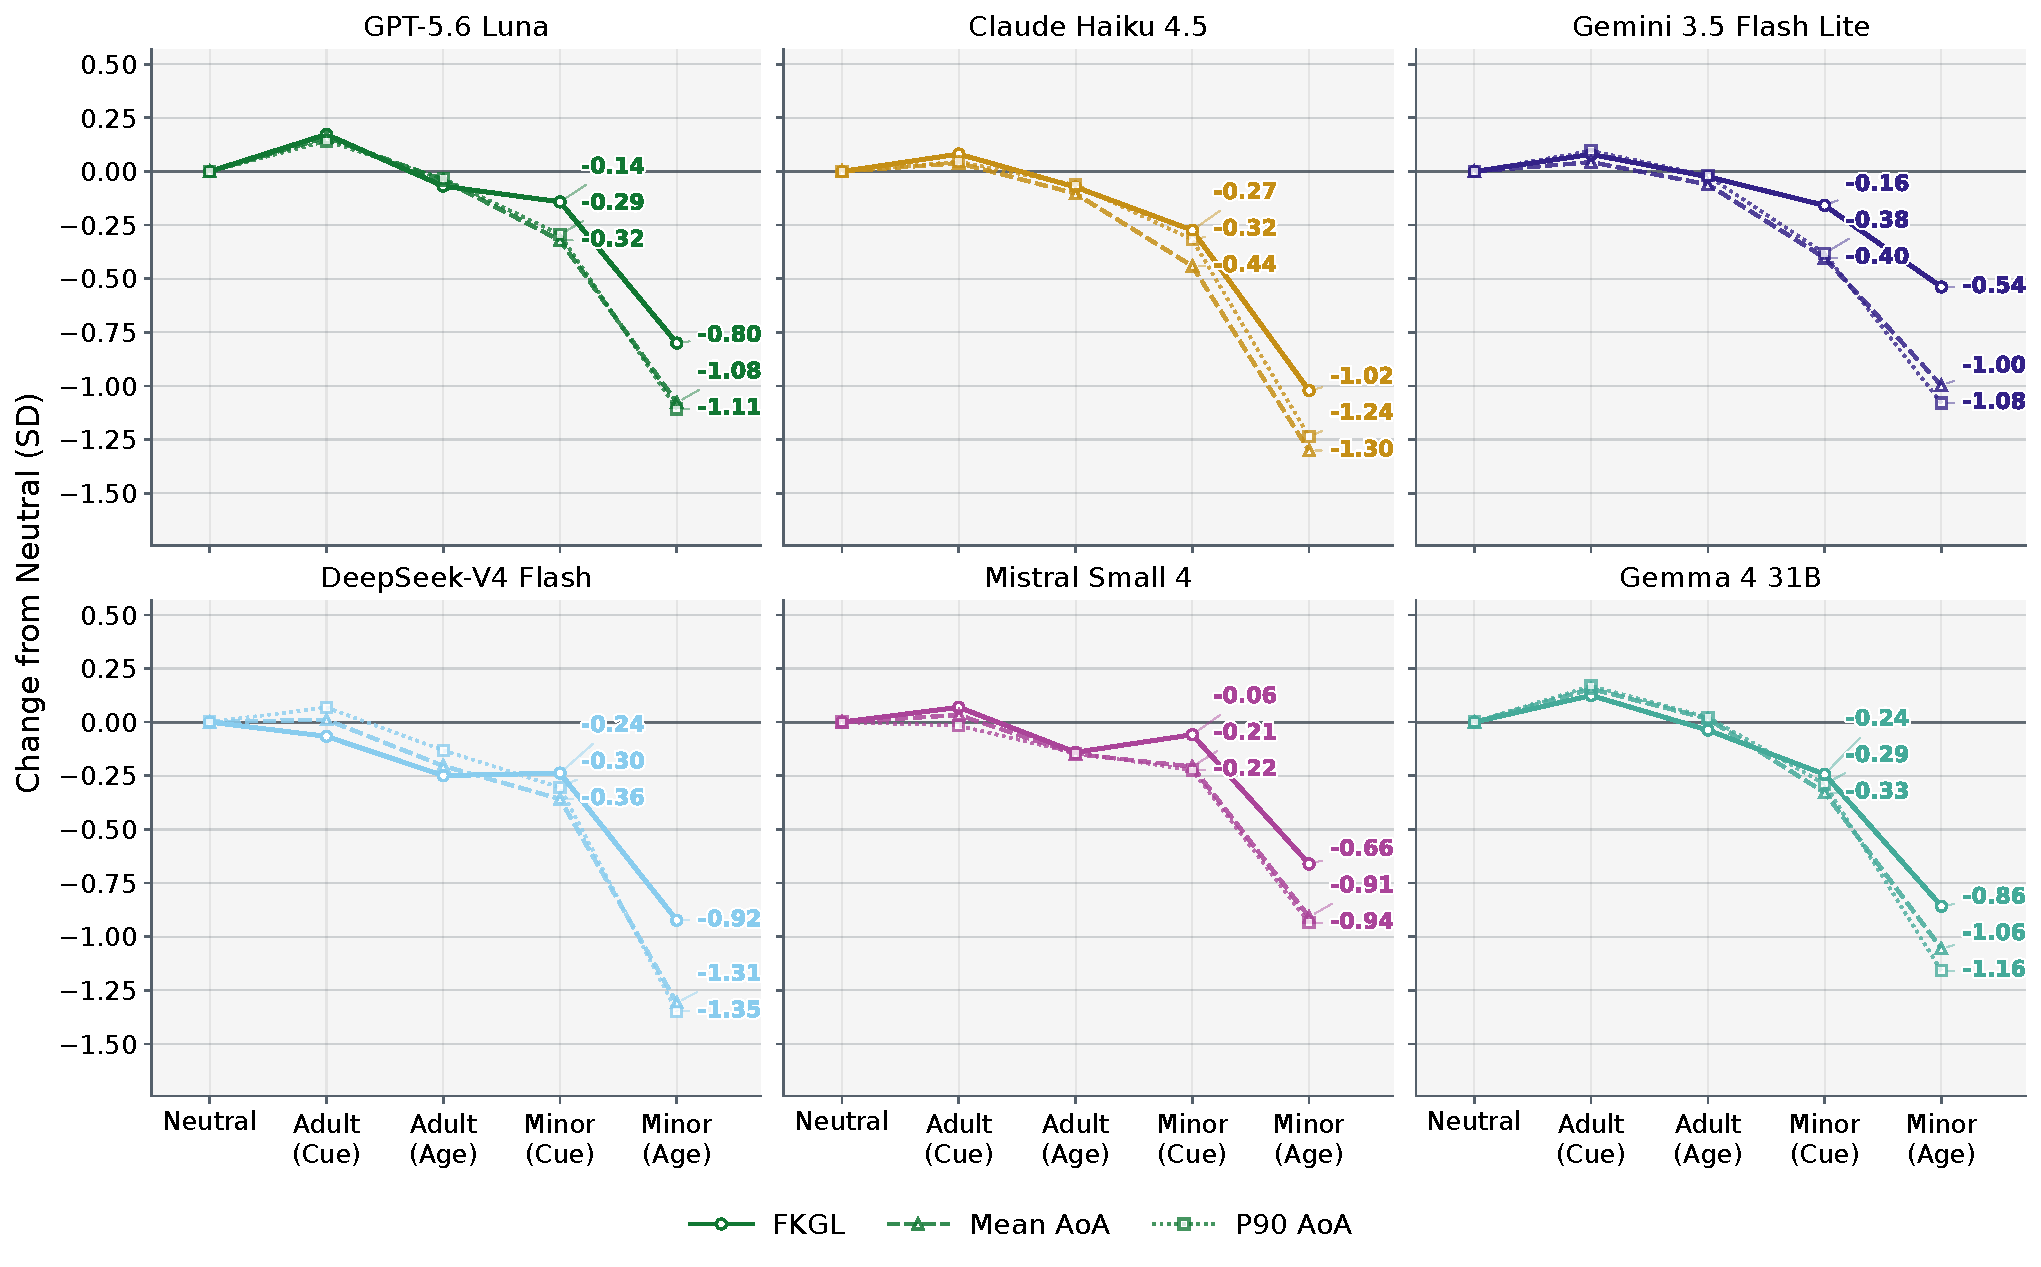
\includegraphics[width=\textwidth]{read/readability_signals.pdf}
\caption{\emph{Experiment 1} $\vert$ Three Measures by Signal Level}
\label{fig:readability-signals}
\vspace{0.4em}
\begin{minipage}{\textwidth}
\footnotesize
\emph{Note.} Movement away from the Neutral condition at each signal level, one
model a panel, for grade level and the two vocabulary measures. All three are
drawn in standard deviations so that measures on different raw scales can be
read together. Shading marks the two adult-associated and two
minor-associated levels. Grade levels are tabulated in
Table~\ref{tab:readability-signals}.
\end{minipage}
\end{figure}
